\documentclass[11pt, xcolor=dvipsnames]{beamer}
\usetheme{Madrid}
\usepackage[utf8x]{inputenc}
\usecolortheme[named=BrickRed]{structure}
\usepackage{xcolor}
\usepackage[ngerman]{babel}

\usepackage{colortbl}

\usepackage{listings}
\lstset{language=Java,
	basicstyle=\footnotesize\ttfamily,
	keywordstyle=\footnotesize\color{blue}\ttfamily,
}

\title{Präfix-Suche}
\author{Christoph Hess}
\begin{document}
	\maketitle
	
	\section{Aufgabenbeschreibung}
	\begin{frame}{Aufgabenbeschreibung}
		\begin{itemize}
			\item Gegeben sei eine Liste von Wörtern, und ein Suchstring. Gesucht sind alle Wörter der Liste, die mit dem Suchstring beginnen.
			
			\item Nicht-Funktionale Anforderungen: Parallele Suche
			\item Inkrementelle Suche, bzw. zwischenspeichern der Suchergebnisse
			\item Nicht erwähnt: Vorberechnung, Zeichensatz, Einfügen von weiteren Wörtern 
		\end{itemize}
	\end{frame}
	\section{Anwendungen}
	\begin{frame}{Anwendungen}
		\begin{itemize}
			\item Autocomplete
			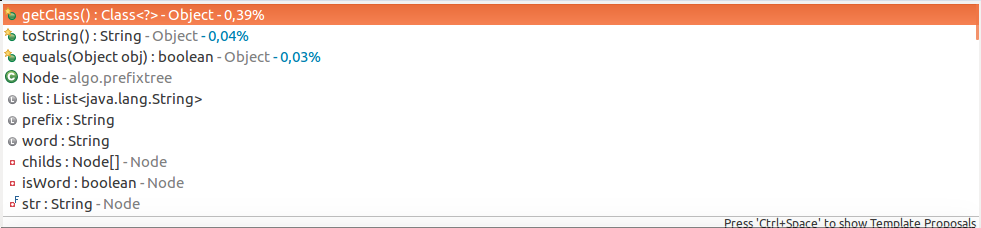
\includegraphics[scale=0.3]{pics/autocomplete.png}
			\item Nomatim-Suche
			
		\end{itemize}
	\end{frame}
	\section{Theorie}
	\begin{frame}{Theoretischer Hintergrund}
	Sei im Weiteren die Liste der Länge $m$, die Länge des Suchstrings $n$, die Ausgabegröße $k$ \\ 
	
	
	\textbf{Untere Schranke ohne Vorberechnung}
		\begin{itemize}
			\item Ohne Vorberechnung muss  jedes Wort mindestens einmal mit maximal $n$ Zeichen betrachtet werden.
			\item Minimale Laufzeit $\Omega(mn)$
		\end{itemize}
		\textbf{Untere Schranke mit Vorberechnung}
		\begin{itemize}
			\item Generierung einer neuen Liste $\Omega(n+k)$ 
			\item Ohne Neu-Generierung einer Liste $\Omega(n)$ (Vorsicht: Speicherplatz!)	
		\end{itemize}
	\end{frame}
	\section{Umsetzung}
	\begin{frame}{Umsetzung - Laufzeitvergleich}
		$m$ Wörter, Länge $l$ des längsten Wortes, Länge $n$ des Suchstrings,\\Ausgabegröße (Wortanzahl) $k$, Anzahl der Prozessoren $p$
		
		\begin{center}
			\begin{tabular}{r|ccc}
		\textbf{Name}	&  Vorberechnung & sequentiell & parallel \\ 
		\hline
		primitiv	& &$O(mn)$ & $O(mn/p)$ \\ 
		PrefixTree	& $O(lm)$ & $O(k+n)$ & \\
		Sort \& BinSearch & $O(parallelsort(m))$ & $O(\log m + k)$ & $O(\log m + k)$
		\end{tabular}
		\end{center} 
	\end{frame}
	
	\begin{frame}{Umsetzung - Zusätzlicher Speicherbedarf}
		$m$ Wörter, Länge $l$ des längsten Wortes, Länge $n$ des Suchstrings,\\Ausgabegröße (Wortanzahl) $k$, Anzahl der Prozessoren $p$
		\begin{center}
		\begin{tabular}{r|ccc}
			\textbf{Name}	&  Vorberechnung & sequentiell & parallel \\ 
			\hline
			primitiv	& &$ O(k)$ & $O(k)$ \\ 
			PrefixTree	& $O(\alpha m)$ & $O(\alpha m + k)$ & $O(\alpha m + k)$ \\
			Sort \& BinSearch & $O(m)$ & $O(m+k)$ & $O(m+k)$
		\end{tabular} 
		\end{center}
	\end{frame}
	
\begin{frame}[fragile]
	\frametitle{Primitive Lösung}
	\ldots als Einzeiler\\
	\textbf{Sequenziell}:
	
	\begin{lstlisting}
public List<String> search(List<String> data, String pattern){
  return data.stream()
    .filter((String s) -> s.startsWith(pattern))
    .collect(Collectors.toList());
}
	\end{lstlisting}
	\textbf{Parallel:}
		\begin{lstlisting}
public List<String> search(List<String> data, String pattern){
  return data.parallelStream()
    .filter((String s) -> s.startsWith(pattern))
    .collect(Collectors.toList());
}
		\end{lstlisting}

Andere Lösungen sind auch vorhanden, nur nicht so kompakt.
\end{frame}

	\begin{frame}
	\frametitle{Sortierung}
	Idee:
	\begin{itemize}
		\item Durch die Sortierung der Eingabedaten ist die Ausgabe konsekutiv darin vorhanden. 
		\item Benutze binäre Suche um den Anfang und das Ende dieses Blocks zu finden.
	\end{itemize}
	Problem: Wie bekomme ich das Ende hin?
	\begin{itemize}
		\item Versuche nächstes Wort des Suchstrings zu ermitteln
%		\item Zeichen sind auch nur Zahlen
%		\item Das letzten Zeichen des Pattern um '1' erhöhen, den Index durch die binäre Suche herausfinden und wieder um '1' verkleinern.  
	\end{itemize}	
	\end{frame}
		
\begin{frame}[fragile]
	\frametitle{Sortierung - NextWord}
	\begin{lstlisting}
public static String nextWord(String pattern) {
  int l = pattern.length();	
  for (int i = l-1; i >= 0; i--) 
    // 127 is the last used position in ascii
    if (pattern.getBytes()[i] > 126) l--;
    else break;
    	
  if (l == 0) return "";	
  int tmpL = Math.max(l - 1,0);
  return pattern.substring(0, tmpL) 
	  + (char)((int)pattern.charAt(tmpL) +1);
}	
	\end{lstlisting}
\end{frame}
	
\begin{frame}[fragile]
	\frametitle{Sortierung - Implementierung}
	Vorberechnung
	\begin{lstlisting}
public void precompute(List<String> data) {
  String[] dataA = new String[data.size()];
  dataA = data.toArray(dataA);
  Arrays.parallelSort(dataA);
  this.data = Arrays.asList(dataA);		
}	
	\end{lstlisting}
	Suchanfrage
	\begin{lstlisting}
public List<String> search(String pattern) {
  if (pattern.length() == 0) return this.data;
	
  int idxL = Collections.binarySearch(data, pattern),
    idxR = Collections.binarySearch(data, nextWord(pattern));
  return this.data.subList(
	idxL < 0 ? -idxL-1 : idxL, 
	idxR < 0 ? -idxR-1 : idxR);
}
	\end{lstlisting}
\end{frame}

	
	\begin{frame}{PrefixTree}
		\begin{itemize}
			\item Basiert auf Bucketsort\\						
			\item Kompression der Pfade für eine geringe Speicherauslastung
		\end{itemize}
		\begin{center}
		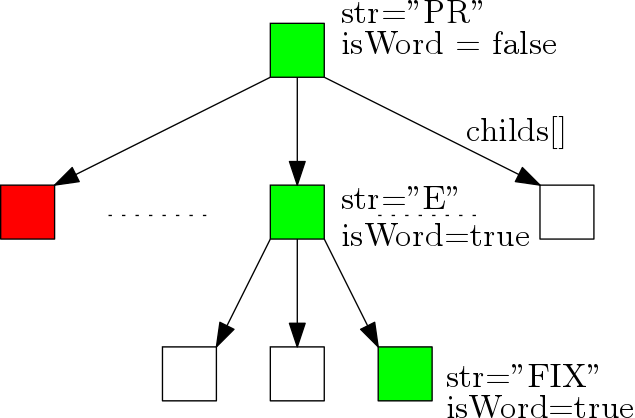
\includegraphics[scale=0.3]{pics/prefixtree.png}
		
		Enthaltene Wörter: PRE, PREFIX, PR\ldots
		\end{center}
		

	\end{frame}
	
	\section{Kritik}
	\begin{frame}{Kritik}
		\centering
		\begin{tabular}{c|cccccc}
			\textbf{Name}	&  Impl. & Geschw. & Platz & parallel & Einfügen & erw. $\mathcal{A}$ \\ 
			\hline
			primitiv	& \cellcolor{green} & \cellcolor{orange}  & \cellcolor{green}& \cellcolor{green} & \cellcolor{green} & \cellcolor{green} \\ 
			Sortieren	& \cellcolor{yellow} & \cellcolor{green} & \cellcolor{yellow} & \cellcolor{yellow} & \cellcolor{yellow} & \cellcolor{green} \\
			PrefixTree & \cellcolor{orange}  & \cellcolor{red} & \cellcolor{red} &\cellcolor{orange} * & \cellcolor{green} & \cellcolor{yellow}
		\end{tabular}\\
		(*) nicht implementiert. 
		
		\begin{itemize}
			\item Die inkrementelle Suche habe ich aufgrund der Geschwindigkeit in eine interaktive Suche umgewandelt.
		\end{itemize}
		%Primitive Suche
		%\begin{itemize}
		%	\item[+] einfach, kurz, gut parallelisierbar
		%	\item[--] langsam auf großen Datensätzen
		%\end{itemize}
		%Sort \& BinSearch
		%\begin{itemize}
		%	\item[+] relativ einfach, schnell
		%	\item[+] Speicherfreundlich
		%	\item[--] Vorberechnung notwendig (parallel möglich)
		%	\item[--] Suche nur auf zwei Prozessoren möglich
		%\end{itemize}
		%PrefixTree
		%\begin{itemize}
		%	\item[+] theoretisch schnell
		%	\item[--] Verwendete Datenstruktur ist nicht speicherfreundlich
		%	\item[--] aufwändiger zu implementieren
		%\end{itemize}
	\end{frame}
	\section{Demo}
	\begin{frame}{Demo}
		\centering

			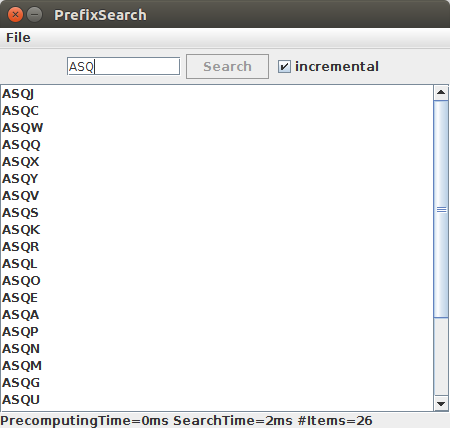
\includegraphics[scale=0.4]{pics/screenshot.png}

			Code und Folien sind versioniert unter:\\
			https://github.com/ch3ss/prefix
	\end{frame}
	\section{Backup}
	\begin{frame}{Backup}
		Inkrementelle Suche:
		\begin{itemize}
			\item Speichern der Ergebnisse und des Suchstrings.
			\item Bei erneuter Anfrage auf Ähnlichkeit prüfen.
			\item Bei Verfeinerung das Zwischenergebnis filtern, ansonsten neu suchen. 
		\end{itemize}
	\end{frame}
\end{document}